\documentclass[conference]{IEEEtran}
\IEEEoverridecommandlockouts
% The preceding line is only needed to identify funding in the first footnote. If that is unneeded, please comment it out.
\usepackage{cite}
\usepackage{amsmath,amssymb,amsfonts}
\usepackage{algorithmic}
\usepackage{graphicx}
\usepackage{textcomp}
\usepackage{xcolor}
\def\BibTeX{{\rm B\kern-.05em{\sc i\kern-.025em b}\kern-.08em
    T\kern-.1667em\lower.7ex\hbox{E}\kern-.125emX}}
\begin{document}

\title{Comparison of $\pi/6$ and $\pi/4$ QPSK Modulation Technique in Wireless Communication Systems\\
{\footnotesize  Digital Modulation - EE5837}\\
{\footnotesize Paper implementation of "Design of an improved QPSK modulation technique in wireless communication systems"}
}

\author{\IEEEauthorblockN{Siddharth Gupta}
\IEEEauthorblockA{\textit{Electrical Engineering, IIT Hyderabad } \\
ee18mtech01003@iith.ac.in}
}

\maketitle

\begin{abstract}
This article is comparison between $\pi$/6 - QPSK and $\pi$/4 -  QPSK modulation techniques. BER (bit error rate) is the comparison criteria between the two schemes. Simulation results of MATLAB shows that the BER performance of proposed $\pi$/6-QPSK is worse than that of conventional $\pi$/4-QPSK modulation scheme which is counter question to[1] as the paper[1] discusses the improved results based on the signal spectral performance of their proposed $\pi/6$-QPSK modulation scheme.

\end{abstract}

\begin{IEEEkeywords}
QPSK, PSK, Modulation, Wireless, $\pi$/4 - QPSK, $\pi$/6 - QPSK 
\end{IEEEkeywords}

\section{Introduction}
Digital transmission system  uses different modulation schemes based on several factors, such as, bandwidth efficiency, power efficiency, low sensitivity to multi path fading and so on[2]. Some of the modulation techniques are ASK, FSK and PSK[3] which changes the carrier amplitude based on amplitude, frequency and phase respectively. PSK is bandwidth efficient and has BER curves of higher types than FSK. Particularly, the performance
of QPSK is better than that of BPSK in case of bandwidth but
it has a limitation of 180º phase shift, which destroy the
constant envelope property [4]. Here we are using PSK modulation schemes, PSK is also called as M-ary PSK. As M increase the density of signal constellation increases which results in better bandwidth efficiency but worse BER. We are explaining QPSK modulation schemes $\pi/4$ and $\pi/6$. for M=4. QPSK stands for Quadrature PSK where quadrature represents M=4. In paper[4] the comparison is made between the two QPSK schemes $\pi/4$ and $\pi/6$, the paper indicates that $\pi/6$-QPSK scheme is better performing in terms of envelop variation since it is less than $\pi/4$- QPSK scheme. 

\section{Theoretical Background}

\subsection{PSK}

In Phase shift keying (PSK), the phase of carrier is changed
with respect to the message data. The general analytical
expression for PSK \cite{b1} can be defined as 

\begin{equation}
s\textsubscript{i}(t)= \sqrt{2E/T} cos[2\pi f\textsubscript{c}t+\phi\textsubscript{i}(t)]
\end{equation}
\begin{math}
\centerline{0\leq t\leq T \; and \;i=1,2,3,...,M}
\end{math}
\vfill
Where, E refers to transmitted signal energy per symbol, T
refers to symbol duration, f\textsubscript{c} is the carrier frequency, $\phi$\textsubscript{i}(t)
denotes the phase of the modulated signal having M discrete
values according to the expression



\subsection{$\pi/6$ QPSK}
In $\pi/6$ QPSK, three constellations are used, which are $\pi/6$
shifted pattern of the QPSK constellation, i.e., successive
constellations are apart by $\pi/6$ degrees. These three
constellations denoted by A, B and C shown in Fig. 1. In $\pi/6$ -
QPSK, constellation is not changed after every symbol. The
constellation selection is depended on input dibit. The
selection of constellation is shown in Table I.

\begin{figure}[htbp]
\centerline{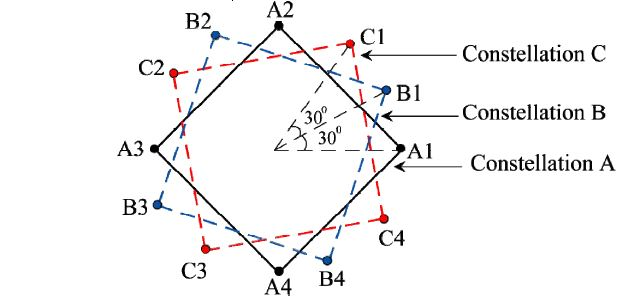
\includegraphics[width=7cm]{const.JPG} }
\caption{Three constellations of proposed $\pi$/6-QPSK scheme}
\label{fig1} 
\end{figure}

\begin{figure}
    \centering
    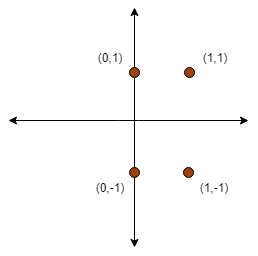
\includegraphics[width=4cm]{const_diagram.png}
    \caption{Constellation diagram after modulation}
    \label{fig2}
\end{figure}
It is clear from Table I that, the $\pi$/6-QPSK is a differential
modulation process, where the transmitted signal is chosen
from one of three QPSK constellations, which are successively
apart by $\pi$/6 degree. Hence, the phase transition between two
successive symbols have the values in between {± $\pi$/6, ±$\pi$2}.
Here, the dibit with corresponding signal phase difference $\Delta \theta$\textsubscript{k} of $\pi$/6-QPSK is shown in Table IV. Therefore, the signal space diagram of $\pi$/6-QPSK is two-dimensional with twelve
message points shown in Fig. 2

    \begin{table}[]
\centering
\begin{tabular}{|c|c|}
\hline
\textbf{Dibit} & \textbf{Constellation Selection} \\ \hline
00 & \begin{tabular}[c]{@{}c@{}}Constellation is unchanged but message point\\ shifted by -90º on existing constellation\end{tabular} \\ \hline
01 & \begin{tabular}[c]{@{}c@{}}Constellation is unchanged but message point\\ shifted by +90º on existing constellation\end{tabular} \\ \hline
10 & \begin{tabular}[c]{@{}c@{}}Constellation is changed, the constellation\\ changing sequence is ACBA cycle and\\ message point shifted by -30º\end{tabular} \\ \hline
11 & \begin{tabular}[c]{@{}c@{}}Constellation is changed, the constellation\\ changing sequence is ABCA cycle and\\ message point shifted by +30º\end{tabular} \\ \hline
\end{tabular}
\bigskip
\caption{ $\pi$/6-QPSK CONSTELLATION SELECTION AND PHASE
TRANSITION FOR DIBIT}
\end{table}


\begin{table}[]
\centering
\begin{tabular}{|c|c|}
\hline
\textbf{Dibit} & \textbf{$\Delta\theta\textsubscript{k}$} \\ \hline
00 & -$\pi/2$ \\ \hline
01 & +$\pi/2$ \\ \hline
10 & -$\pi/6$ \\ \hline
11 & +$\pi/6$ \\ \hline
\end{tabular}
\bigskip
\caption{ SIGNAL PHASE DIFFERENCE OF $\pi$/6-QPSK SCHEME}
\end{table}

\subsection{$\pi/6$ Modulator}
$\pi/6$ QPSK Modulator
The $\pi/6$QPSK is a deferentially encoded and decoded system.
The $\pi/6$-DQPSK modulator is shown in Fig.9. The differential
encoder of $\pi/6$ DQPSK modulator encodes $I_{k}$ and $Q_{k}$ into
signal $u_{k}$ and $v_{k}$ according to the following rules:

\\

\begin{math}



    u_{k} = 1/2\sqrt{2}[u_{k-1}(\sqrt{3+3I_{k}})-v_{k-1}Q_{k}(\sqrt{5-3T_{k}})]
    \\

    v_{k} = 1/2\sqrt{2}[u_{k-1}Q_{k}(\sqrt{5-3T_{k}})+v_{k-1}(\sqrt{3+3I_{k}})

\end{math}

\subsection{$\pi/6$ De-Modulator}

It is seen in Fig. 1 that, the signal space diagram of $\pi/6$QPSK
has twelve message points. However, at instant, $\pi/6$QPSK
works only on four message points and the decision region for
selecting symbol of $\pi/6$QPSK is shown in Fig. 2. Therefore,
in $\pi/6$QPSK, the following decisions can be made as,

\begin{equation}
  I_{k}=\left\{
  \begin{array}{@{}ll@{}}
    1, & \text{if}\ \sqrt{3}x_{k}>|y_{k}| \\
    0, & \text{if}\ \sqrt{3}x_{k}<|y_{k}|
  \end{array}\right.
\end{equation} 
\begin{equation}
    Q_{k}=\left\{
  \begin{array}{@{}ll@{}}
    1, & \text{if}\ y_{k}>0 \\
    0, & \text{if}\ y_{k}<0
  \end{array}\right.
\end{equation}
Where, $|y_{k}|$ is the absolute or modulus value of $y_{k}$.

\begin{figure}[htbp]
\centerline{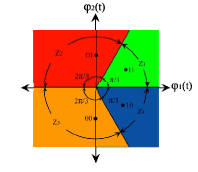
\includegraphics[width=5cm]{decision_region.png} }
\caption{Decision region of $\pi/6$QPSK for symbol selections.}
\label{fig2}
\end{figure}

\section{Results}
Following results are obtained from MATLAB simulation where Fig. 1 is representing the BER curve of 1000 samples for $\pi/4$ QPSK scheme and $\pi/6$ QPSK scheme. Similarly the same is represented in Fig. 2 for 10000 samples and, for 10\textsuperscript{6} samples in Fig. 3

\begin{figure}[htbp]
\centerline{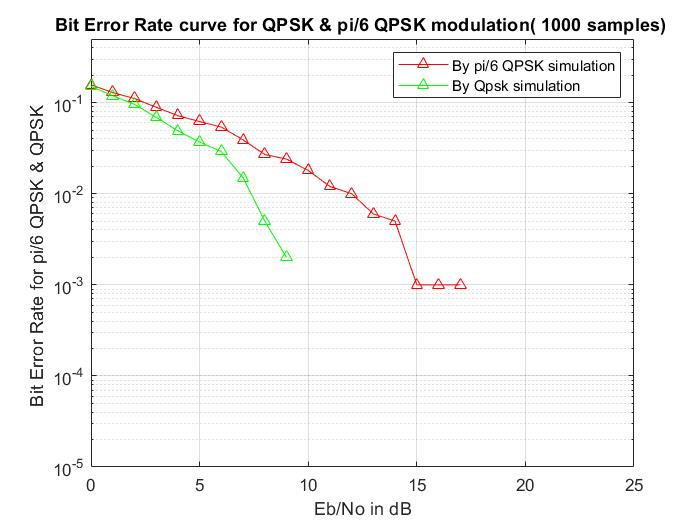
\includegraphics[width=5cm]{1.jpg} }
\caption{BER curve for 1000 samples.}
\label{fig1}
\vspace{0.5cm}

\centerline{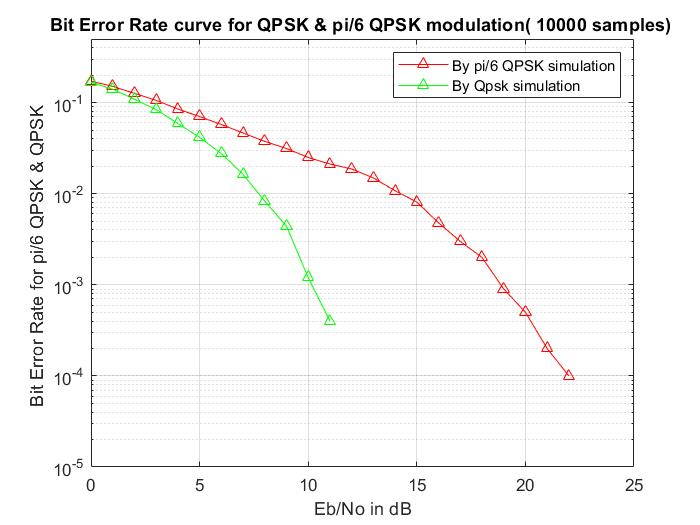
\includegraphics[width=5cm]{10.jpg} }
\caption{BER curve for 10000 samples.}
\label{fig2}
\vspace{0.5cm}
\centerline{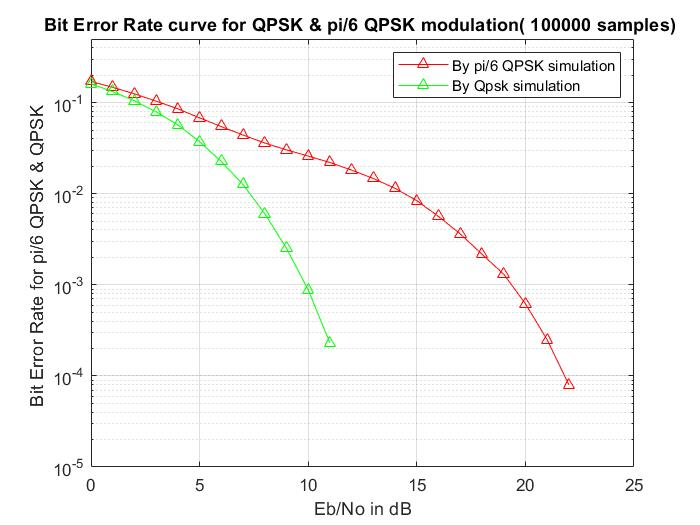
\includegraphics[width=5cm]{100.jpg} }
\caption{BER curve for 100000 samples.}
\label{fig3}
\end{figure}


\section{Conclusion}

Figure 3, 4 and 5 represents BER curve of both the schemes. Bit error rate for $\pi/6$ QPSK scheme is much higher than the  $\pi/4$ QPSK scheme for same (Eb/No) signal to noise ratio, for all the three iterations over different samples (1000,10000,100000). For 100000 samples the drop is around 10\textsuperscript{-4} at 23db  for $\pi/6$ QPSK and   same BER is attained at 12db for $\pi/4$ QPSK, hence the performance of $\pi/4$ QPSK is better than $\pi/6$ QPSK scheme.


\begin{thebibliography}{00}
\bibitem{b1}M. A. N. Chowdhury, M. R. U. Mahfuz, S. H. Chowdhury and M. M. Kabir, "Design of an improved QPSK modulation technique in wireless communication systems," 2017 3rd International Conference on Electrical Information and Communication Technology (EICT), Khulna, 2017, pp. 1-6
\bibitem{b2} D. Sai Brunda, B. Geetha Rani, “Design of QPSK Digital Modulation
Scheme Using Turbo Codes for an Air Borne System”, International
Journal of Advanced Research in Computer and Communication
Engineering (IJARCCE),vol. 5, issue 8, August 2016.
\bibitem{b3}Simon Haykin, Digital Communication, Wiley Press, 2013
\bibitem{b4}J. Webber, N. Dahnoun, Implementing a $\pi/4$-Shifted DQPSK Baseband
Modem Using the TMS320C50, ESIEE, Paris, September 1996

\end{thebibliography}

\end{document}
